\documentclass{llncs}

\usepackage{url}
\usepackage{graphicx}
\usepackage{listings}
\usepackage{verbatim}
\usepackage[lined,linesnumbered,algochapter]{algorithm2e}
\usepackage{tikz}
\usetikzlibrary{arrows,automata}
\usepackage{xspace}
\usepackage{todonotes}          % Package for working draft comments
\usepackage{hyperref}           % Package for hyperlink references in the document

\usepackage[english]{babel}

\setcounter{secnumdepth}{2}
\setcounter{tocdepth}{3}

% define custom macros for specific formats or names
\newcommand{\uml}[1]{\texttt{#1}}
\newcommand{\cd}{\textsf{Class Diagram}}

\lstnewenvironment{lstsingle}[1][]%
 {\noindent\minipage{\linewidth} 
  \vspace{0.5\baselineskip}
  \lstset{#1}}
 {\endminipage}

%Colors for general listings
\definecolor{mygreen}{rgb}{0,0.6,0}
\definecolor{mygray}{rgb}{0.5,0.5,0.5}
\definecolor{mymauve}{rgb}{0.58,0,0.82}
%Colors for JSON listings
\colorlet{punct}{red!60!black}
\definecolor{background}{HTML}{EEEEEE}
\definecolor{delim}{RGB}{20,105,176}
\colorlet{numb}{magenta!60!black}

\lstset{ %
   backgroundcolor=\color{background},   % choose the background color; you must add \usepackage{color} or \usepackage{xcolor}
   basicstyle=\small\ttfamily,        % the size of the fonts that are used for the code
%   breakatwhitespace=false,         % sets if automatic breaks should only happen at whitespace
%   breaklines=true,                 % sets automatic line breaking
  captionpos=b,                    % sets the caption-position to bottom
  commentstyle=\color{mygreen},    % comment style
%   deletekeywords={...},            % if you want to delete keywords from the given language
%   escapeinside={\%*}{*)},          % if you want to add LaTeX within your code
%   extendedchars=true,              % lets you use non-ASCII characters; for 8-bits encodings only, does not work with UTF-8
   frame=lines,                    % adds a frame around the code
%   keepspaces=true,                 % keeps spaces in text, useful for keeping indentation of code (possibly needs columns=flexible)
  columns=fixed,
  keywordstyle=\color{mymauve},       % keyword style
  stringstyle=\color{blue},
%   morekeywords={*,...},            % if you want to add more keywords to the set
  numbers=left,                    % where to put the line-numbers; possible values are (none, left, right)
  numbersep=5pt,                   % how far the line-numbers are from the code
  numberstyle=\scriptsize\color{mygray}, % the style that is used for the line-numbers
%   rulecolor=\color{black},         % if not set, the frame-color may be changed on line-breaks within not-black text (e.g. comments (green here))
 showspaces=false,                % show spaces everywhere adding particular underscores; it overrides 'showstringspaces'
 showstringspaces=false,          % underline spaces within strings only
 showtabs=false,                  % show tabs within strings adding particular underscores
%   stepnumber=2,                    % the step between two line-numbers. If it is 1, each line will be numbered
  tabsize=2,                       % sets default tabsize to 2 spaces
%   title=\lstname                   % show the filename of files included with \lstinputlisting; also try caption instead of title
}


\begin{document}
\renewcommand{\thelstlisting}{\arabic{lstlisting}}
\pagestyle{plain}
\pagenumbering{roman}

\title{Refactoring UML models: Co-refactoring fUML conform class diagrams and activity diagrams}

\author{Sebastian Geiger (1127054) \and Kristof Meixner (9725208)}
\institute{Business Informatics Group\\Vienna Technical University}
\maketitle

\begin{abstract}
In this work we will present ideas and concepts for the refactoring of fUML conform UML models. The main contribution of this work is 
the extension of existing UML refactorings. Our refactorings cover not only the static aspect of UML such as class diagrams but consider 
the co-refactoring of the dynamic parts such as activity diagrams as well. In this work we will present basic concepts for the refactoring 
of models with EMF and show how model semantics can be preserved through the use of OCL constraints. Furthermore we present our toolchain 
and the technologies of EMF (in particular Ecore and OCL) and how we used them for the co-refactoring of fUML conform UML models. We 
also present a discussion of EMF Refactor, which shows how such refactorings can be made available in the Eclipse GUIs such as the UML 
tree editor or the Papyrus UML editor.
\end{abstract}

\tableofcontents
\newpage

\pagenumbering{arabic}

\section{Introduction}
% INTRODUCTION Models are getting more important in model-based software development, model-driven software development,
% model-driven architecture Models thus need to have a good quality

Model-based software development or model-driven software development is not only an extensive field of research but
also receives increased attention from the industry. Nowadays models are not only used as visual explanations of
software concepts but as source for the development process itself. Thus models need to provide an abstraction of
the represented domains in a high quality. Mohagheghi \textit{et al.} \cite{DBLP:journals/infsof/MohagheghiDN09} discussed 
quality attributes like \textit{Correctness}, \textit{Completeness} and \textit{Consistency} of models in their work.

% UML is a modelling language for models provided by the OMG that supports various types of models

To represent models in a more formal way the \textit{Object Management Group} (OMG) developed the \textit{Unified Modeling Language} (UML) 
\cite{man:UML} which by now advanced to an industry standard for 
modeling. UML provides an abstract syntax of the modeling concepts and rules how to combine them, an explanation 
of the semantics of the concepts as well as a specification of the notation elements in human-readable form.
Build on these common concepts models can be preserved over time and even be reused due to their formalized semantics. Nevertheless models 
might have to be revised over the lifecycle of the software. With todays trend to more agile software 
development such as eXtreme Programming \cite{DBLP:journals/computer/Beck99} or Scrum \cite{DBLP:journals/software/RisingJ00} 
changes on models have to be even more efficient which brings refactoring of models into the focus of research.

% Refactoring is behavior preserving changing that should also improve quality

Refactoring is a technique that originates from source code development but can also be applied to model engineering.
The goal is to introduce behavior preserving changes \cite{mast:REFOOF} that increase the quality and understandability
of the models.

% Refactoring must preserve the behavior of all model types

While refactoring source code and textual code respectively applies to a single type of representation, in UML different
types of diagrams exist to represent various aspects of the models. This makes behavior preserving refactoring even harder 
as it needs to span over those different types of diagrams and semantics.

% Behaviour preservation can be tested statically or dynamically UML can be analysed statically fUML is a modelling
% language for models provided by the OMG that also allows execution and thus can be analysed dynamically

Different approaches exist to prove the semantic preservation of refactorings. One is the static analysis of
UML models via the \textit{Object Constraint Language} (OCL) \cite{man:OCL} to assert different properties of the UML model, both before 
and after the refactoring. Another way is to verify that models can be executed and to compare 
different attributes of the execution like input and output values, execution traces or states of the 
original and refactored models. The OMG introduced a foundational subset 
of UML metamodel concepts abbreviated fUML \cite{man:FUML} and precisely defined the semantics for their execution. Thanks 
to this standard compliant UML models can be transformed to an executable form. 
Furthermore in \cite{DBLP:conf/icse/Mayerhofer12} Mayerhofer \textit{et al.} proposed a framework based on fUML that is able to execute
and debug models that conform to fUML.

% our approach is to combine both

The goal of this work is to introduce refactorings for fUML models, examine the requirements for co-refactoring of the
corresponding diagram types and define which co-changes have to be performed to preserve the behavior. Our approach to
verify the semantic preservation and the correctness of the models is twofold. On the one hand we use OCL pre- and postconditions
\cite{rob99} to determine whether a refactoring can be applied and whether the models are semantically correct afterwards.
On the other hand the models have to stay executable after the changes, if they are executed with the same input data.

% we present a motivating example (class and activity diagrams) we provide some refactorings that target bothe diagram
% types we provide a how to test statically and dynamically, then refactor and retest we provide a toolchain

% we provide some related work we provide a conclusion

The rest of the work is structured as follows. Section \ref{sec:motivation} gives an introduction to fUML and shows how 
the preservation of semantics can be achieved during refactoring. 
Section \ref{refactoring-examples} describes a selection of useful refactorings inspired by Fowler \cite{fow99} and 
Markovic and Baar \cite{DBLP:journals/sosym/MarkovicB08} and their effects on class diagrams as
well as activity diagrams. We also provide a motivating example of a model that is used throughout the paper. In Section 
\ref{sec:fuml-refactoring} we show which pre- and postcondition are needed for the refactorings and
how we refactor the models. In Section \ref{sec:toolchain} we describe the toolchain that we use to define the models, 
implement a set of refactorings and test them. Section \ref{sec:limitations} describes which limitations our work has. 
Related work is covered in Section \ref{sec:relatedwork} and a conclusion is drawn in 
Section \ref{sec:conclusion} to summarize the paper.

% what is refactoring and what does it mean in the context of models?
% what is fuml? what does fuml consist for diagram types?
% what is ocl? why do we use it and what for?

%fUML adds semantics to UML models that make it possible to create semantically closed models which can be executed on the model level. With
%fUML classic refactorings are not enough to refactor those models as they do not support the refactoring of the dynamic aspects of models
%such as activity diagrams.

\section{Motivation}
\label{sec:motivation}
% what do we want to achieve?
fUML is a subset of UML for which additional semantics are defined such that models can be executed. The subset contains concepts
of the packages \textit{Classes}, 
\textit{CommonBehaviors}, \textit{Activities} and \textit{Actions}, which basically means that it is possible to create 
\textit{class diagrams} and \textit{activity diagrams} with fUML. At the same time it means that UML models which conform to fUML
are also executable.

If a refactoring 
is performed on a UML model such as a class diagram, then any activity diagram which is releated to the class diagram, has 
to be checked and possibly changed as well. In Section \ref{sec:fuml-refactoring} we will present some examples of fUML 
activity diagrams and present the implications that result from changing class 
diagrams (a procedure called \textit{co-refactoring}).

Since a refactoring changes the structure of a model it is important to ensure that all changes maintain the original 
semantics of the model. Violating this requirement can result in models with either a different behavior, or in models 
which can no longer be executed. To ensure semantic preservation, two main techniques can be used. First, the refactoring 
can be broken down into smaller steps, each of which either guarantees to preserve the semantics of the model or makes it 
easier to verify that this is the case. Second, logical constraints can be used to limit refactorings on models to only 
those cases where semantic preservation can be ensured. For this purpose pre- and postconditions are specified with OCL 
constraints. A refactoring is then only applied if the original model satisfies the precondition before the refactoring is 
applied and the postcondition after the refactoring has been completed. Such constraints must be individually specified 
for each kind of refactoring that is to be performed. In this paper we introduce and discuss different OCL constraints 
for the refactorings that we introduce.

Refactorings are only useful if they can be easily applied to the models through an easy to use process such as a 
graphical front end. EMF Refactor\footnote{\url{http://www.eclipse.org/emf-refactor/}} allows the integration of 
refactorings into editors such as the UML tree editor or 
the Papyrus\footnote{\url{http://www.eclipse.org/papyrus/}} UML editor. EMF Refactor provides a Java API as well as a module 
concept to integrate refactorings. We will discuss the use 
of Papyrus and EMF Refactor as part of our tool chain presentation.

%TODO: Maybe discuss emf.refactor as part of future work?

% Why is it interesting to refactor models
% Why is it important in fUML that models remain consistent -> to preserve executability
% It is possible to use pre and post conditions in OCL to guarantee the semantic preservation of models during refactorings.

\section{Refactoring examples}
\label{refactoring-examples}
% take model refactorings of markovic paper
% insurance example
% create example that supports all proposed refactorings

This section covers some refactorings of fUML models as well as a fUML model which we use as an example for this work. 
Markovic \cite{DBLP:journals/sosym/MarkovicB08} presented a list of refactorings for class 
diagrams and co-refactoring of OCL constraints. However they do not consider other diagram types and possible co-refactorings between 
them. Nevertheless we use this catalog as a starting point and adapt it for our use case. 

\begin{figure}[h!t]
 \centering
 \begin{tabular}[]{l | c | c | c}
  \shortstack{Class diagram\\refactoring} & \shortstack{Abstract syntax\\changes} & \shortstack{Activity diagram\\co-refactoring} & Implemented\\
  \hline
  Encapsulate property & Yes & Yes & Yes\\
  Extract class & Yes & Yes & No\\
  Pull up association end & Yes & Yes & No\\
  Pull up properties & Yes & Yes & Yes\\
  Pull up operation & Yes & No & Yes\\
  Extract superclass & Yes & No & Yes\\
  Remove unused class & Yes & No & No\\
  Rename class & No & No & Yes\\
  Rename operation & No & No & Yes\\
  Rename property & No & No & Yes\\
 \end{tabular}
 \caption{Considered refactorings}
 \label{fig:refactoringlist}
\end{figure}

The resulting list of 
refactorings which we plan to evaluate and implement is shown in Figure \ref{fig:refactoringlist}. 
The first column (\textit{Class diagram refactoring}) displays the name of the refactoring as used in \cite{DBLP:journals/sosym/MarkovicB08}, but adapted to the 
concept names used in UML\footnote{E.g. instead of \textit{attribute} we use the \textit{property} in the name of the refactoring}. 
The second column (\textit{Abstract syntax change}) indicates whether the abstract syntax changes due to the refactoring.
Finally the third column (\textit{Activity diagram co-refactoring}) shows whether we need to co-refactor the corresponding activity diagrams 
in parallel to the changes in the class diagram.

If we apply for example a rename refactoring the abstract syntax does not change because the concepts are linked 
by reference and the new name will automatically ``propagate'' to the other concepts. Thus there is no need to 
co-refactor the activity diagrams. Another example would be the \textit{encapsulate property} refactoring which 
changes the abstract syntax as new operations are introduced and the visibility of the property is changed. This 
has also effects on the activity diagram where several actions accessing the property might have to be changed. 
A more detailed explanation of co-refactorings is given in Section \ref{sec:fuml-refactoring} together with the introduction of each 
refactoring.

\begin{figure}[h!t]
 \centering
 \makebox[\textwidth]{
 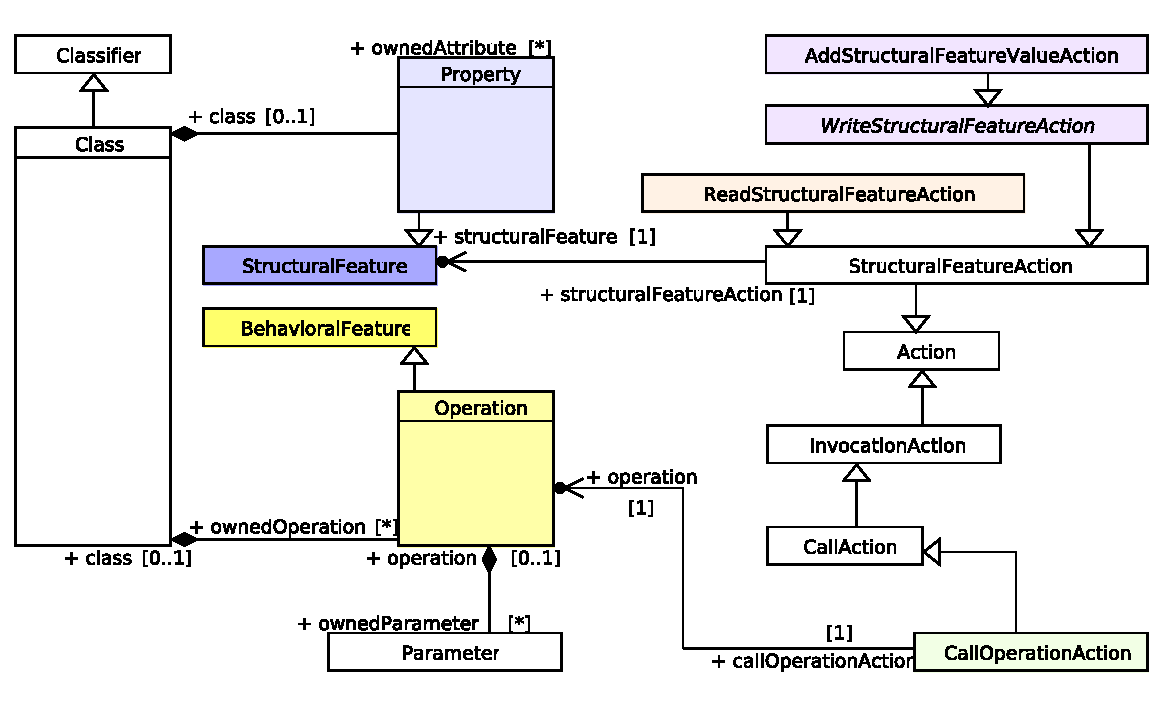
\includegraphics[scale=0.65]{images/Model_Model_Classifiers}
 }
 \caption{Abstract syntax for used class concepts in \textit{fUML}}
 \label{fig:fuml1}
\end{figure}

In order to demonstrate how the presented refactorings affect both class and activity diagrams we will introduce an example 
model from the insurance domain. For a better understanding of the abstract syntax we first show the most relevant parts of the fUML 
subset for our example. Figure \ref{fig:fuml1} explains how the meta-model concepts \texttt{Property}, which is a subclass of 
\texttt{Structural\-Feature}, and \texttt{Operation}, which is a \texttt{Behavioral\-Feature}, are linked to the \texttt{Class}. 
Furthermore is shows that \texttt{Operation} owns zero or more \texttt{Parameter}. It also shows the hierarchy of 
the most relevant actions. Important to mention is the \texttt{Call\-Operation\-Action} which holds a single \texttt{Operation}, 
and the \texttt{Structural\-Feature\-Action}, which holds a single \texttt{Structural\-Feature}. To better recall the abstract 
concepts we colored them and used the color for the diagrams in the paper.

Figure \ref{fig:classdiagramcomplex} shows our example class diagram of an insurance company with relevant properties and operations. 
In our case there are different domain objects. A company administers different customers and employs some employees. Further more the \
company sells insurance policies where trucks and cars can be added and insured for a certain period. Customers can hold such insurance 
policies that are signed by an employee to verify the correctness.

\begin{figure}[h!t]
 \centering
 \makebox[\textwidth]{
 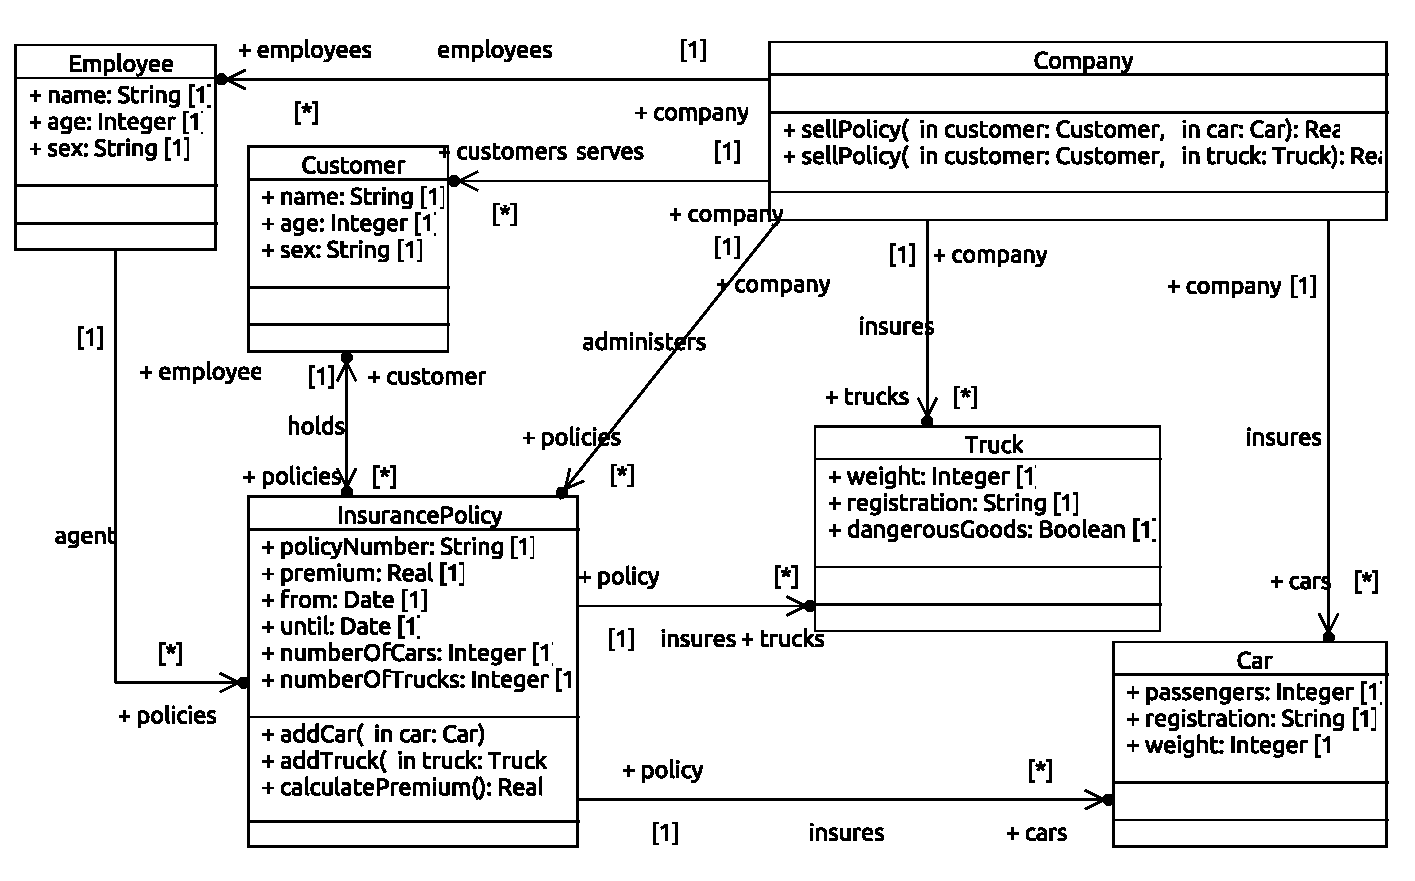
\includegraphics[scale=0.65]{images/insurance/Model_Model_ClassDiagram.PDF}
 }
 \caption{Insurance class diagram before refactoring}
 \label{fig:classdiagramcomplex}
\end{figure}

This class 
diagram would benefit from several possible refactorings such as an \textit{extract superclass} which can be applied to both \texttt{Car} 
and \texttt{Truck} to extract a \texttt{Vehicle} class. An \textit{extract class} refactoring can be used on \texttt{InsurancePolicy} to 
extract the \texttt{from} and \texttt{until} dates into an own \texttt{InsurancePeriod} class. As part of the 
\textit{extract superclass} refactoring two additional refactorings namely \textit{pull up property} and \textit{pull up operation} are 
used to move the identical properties and operations of both classes to the new superclass. As the 
properties \texttt{weight} and \texttt{registration} are public, we can use \textit{encapsulate field} to set their visibility to private and 
provide getter and setter operations. Finally a new operation \texttt{addVehicle} can be introduced and the \texttt{addTruck} as well as 
the \texttt{addCar} operation can be removed with \textit{remove operation}\footnote{\textit{add operation} and \textit{remove operation} are not covered by our paper}. 
Figure \ref{fig:classdiagramcomplexRef} shows the class diagram resulting from the refactoring.

\begin{figure}[h!t]
 \centering
 \makebox[\textwidth]{
 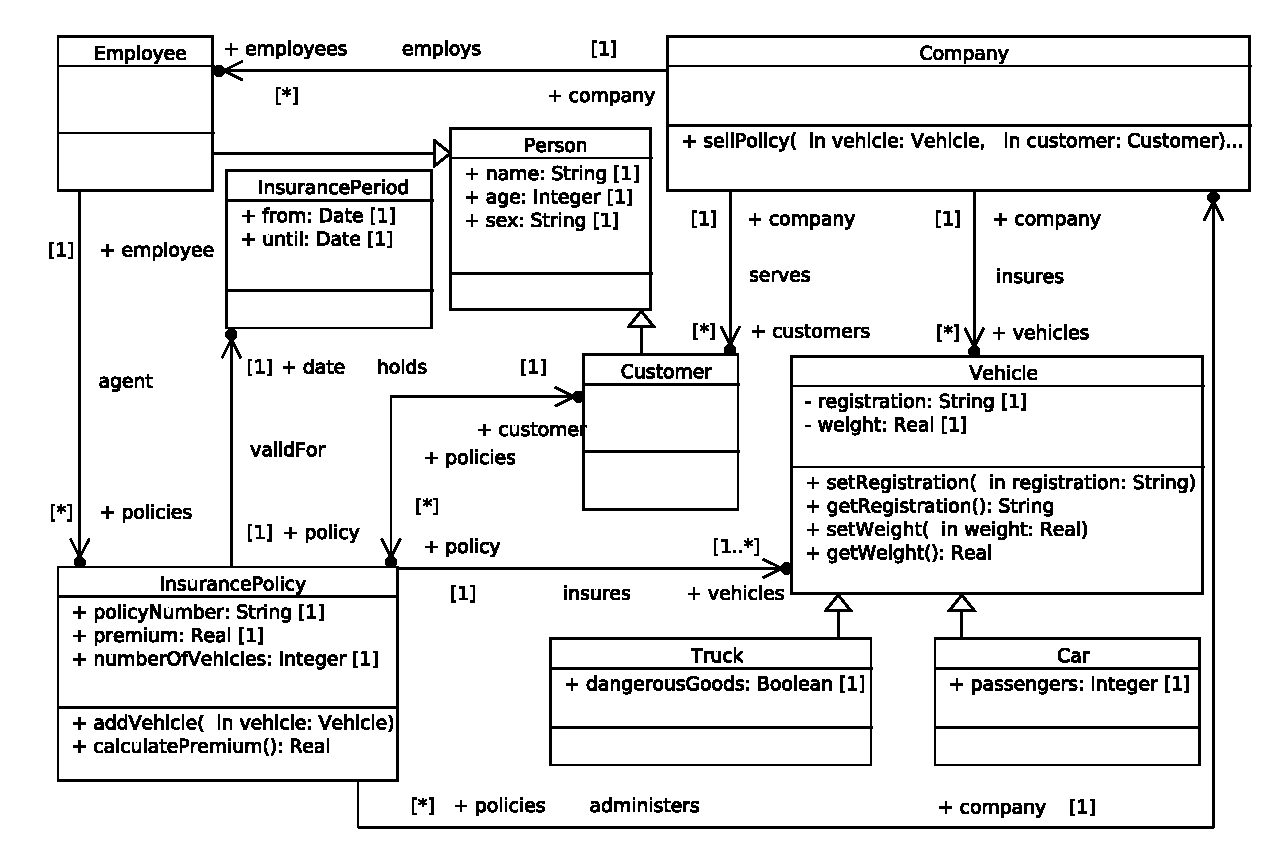
\includegraphics[scale=0.65]{images/insurance_ref/Model_Model_ClassDiagram}
 }
 \caption{Insurance class diagram after refactoring}
 \label{fig:classdiagramcomplexRef}
\end{figure}

For each of the operations in the \texttt{InsurancePolicy} class a separate activity diagram exists which defines the behavior 
of the respective operation. As some of them are quite similar we will present only the diagrams for \texttt{addCar} in Figure 
\ref{fig:addCar} and \texttt{calculatePremium} in  Figure \ref{fig:calculatePremium}.

The activity for the \texttt{addCar} operation works as follows. It reads the policy with a \texttt{Read\-Self\-Action}, takes the 
car as a parameter and uses the \texttt{Add\-Structural\-Feature\-Value\-Action} to add the car to the insurance policy. In parallel 
it reads the number of cars in the policy with \texttt{Read\-Structural\-Feature\-Value\-Action}, specifies an integer
with a value of '1' with 
a \texttt{Value\-Specification\-Action}, adds the numbers with a \texttt{Call\-Behavior\-Action} and writes it back to the 
\texttt{numberOfCars} variable with another \texttt{Add\-Structural\-Feature\-Value\-Action} that replaces the old value.

The \texttt{calculatePremium} activity is more complex, it calculates the insurance premium as described below:

\begin{itemize}
 \item Read the policy with a \texttt{Read\-Self\-Action}.
 \item Read the number of cars and trucks with \texttt{Read\-Structural\-Feature\-Value\-Action}.
 \item Add the two numbers up with a \texttt{Call\-Behavior\-Action}, which invokes the opaque behavior 'add'.
 \item Multiply the result in a \texttt{Call\-Behavior\-Action} with a base premium value specified in a \texttt{Value\-Specification\-Action}.
 \item Read the age of customer of the policy with two actions of type \texttt{Read\-Structural\-Feature\-Value\-Action} in a row.
 \item Decide whether the age of a customer is below a certain age and define a base value or supplement with a \texttt{Value\-Specification\-Action}.
 \item Multiply the value and the result of the calculation above and return it.
\end{itemize}

\begin{figure}[h!t]
 \centering
\makebox[\textwidth]{
 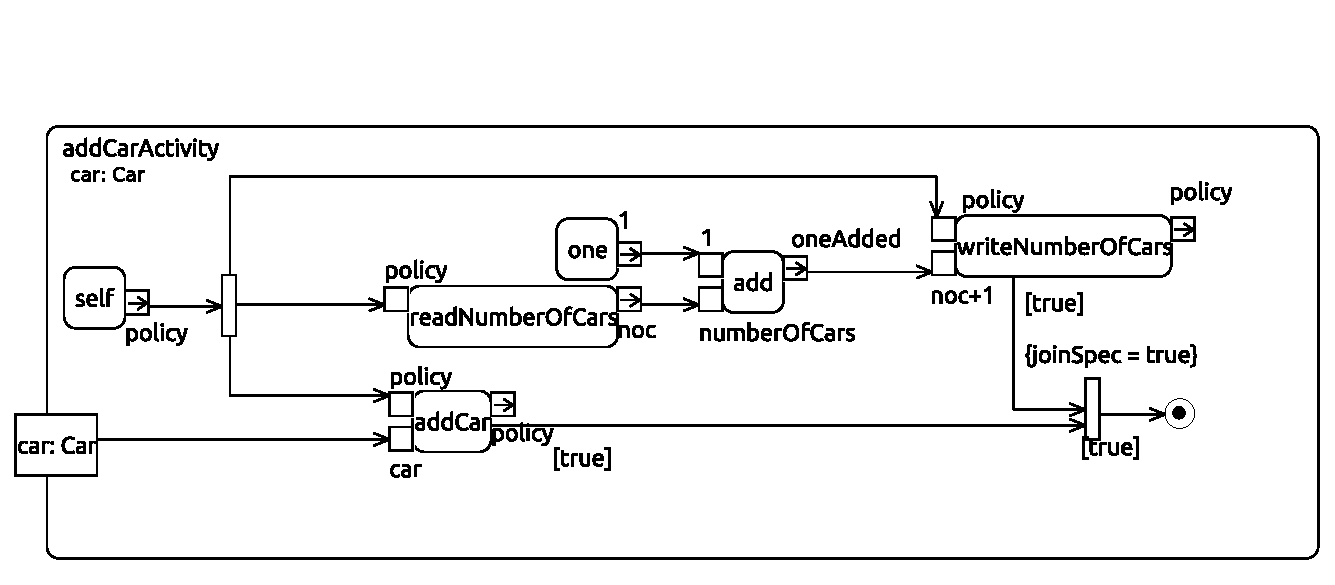
\includegraphics[scale=0.7]{images/insurance/Activity_addCarActivity_addCarActivity}
}
 \caption{Activity diagram of operation \texttt{addCar} before refactoring}
 \label{fig:addCar}
\end{figure}

\begin{figure}[h!t]
 \centering
\makebox[\textwidth]{
 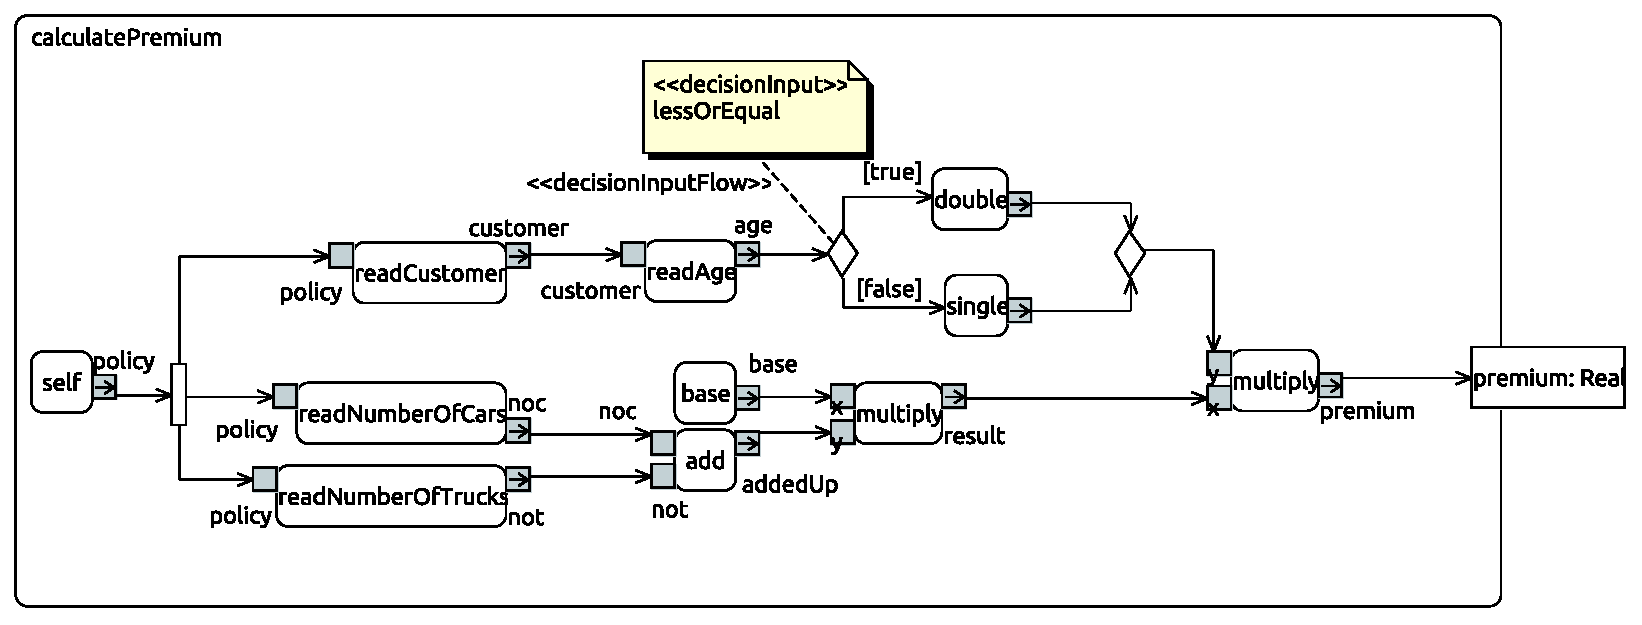
\includegraphics[scale=0.6]{images/insurance/Activity_calculatePremium_calculatePremium}
}
 \caption{Activity diagram of the operation \texttt{calculatePremium} before co-refactoring}
 \label{fig:calculatePremium}
\end{figure}

Figure \ref{fig:calculatePremiumRef} shows how the activity diagram of the operation \texttt{calculatePremium} benefits from a refactoring of the corresponding 
class diagram. Additionally a new activity diagram for the \texttt{addVehicle} operation instead of the old 
\texttt{addCar} and \texttt{addTruck} diagrams was created shown in Figure \ref{fig:addCarRef}. It is rather obvious 
that the complexity of both diagrams decreased on the visual level which helps interested parties to better understand the 
model.

\begin{figure}[h!t]
 \centering
 \makebox[\textwidth]{
 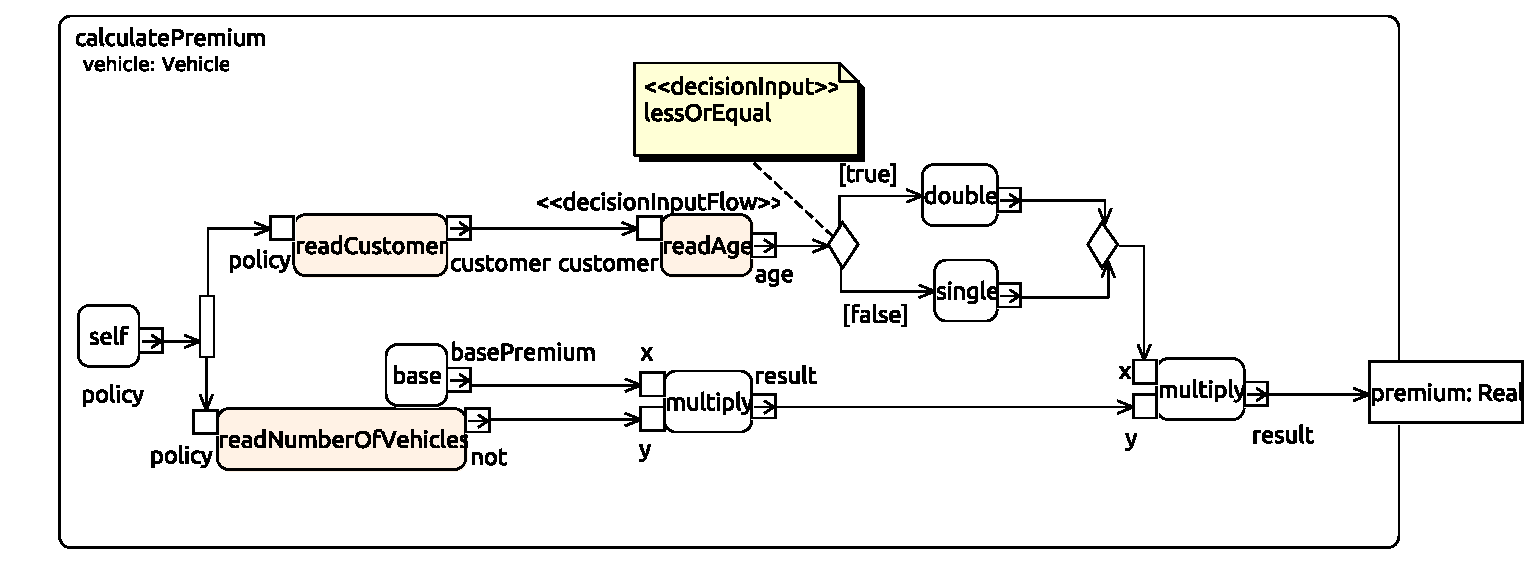
\includegraphics[scale=0.6]{images/insurance_ref/Activity_calculatePremium_calculatePremium}
 }
 \caption{Activity diagram of the operation \texttt{calculatePremium} after co-refactoring}
 \label{fig:calculatePremiumRef}
\end{figure}

\begin{figure}[h!t]
 \centering
 \makebox[\textwidth]{
 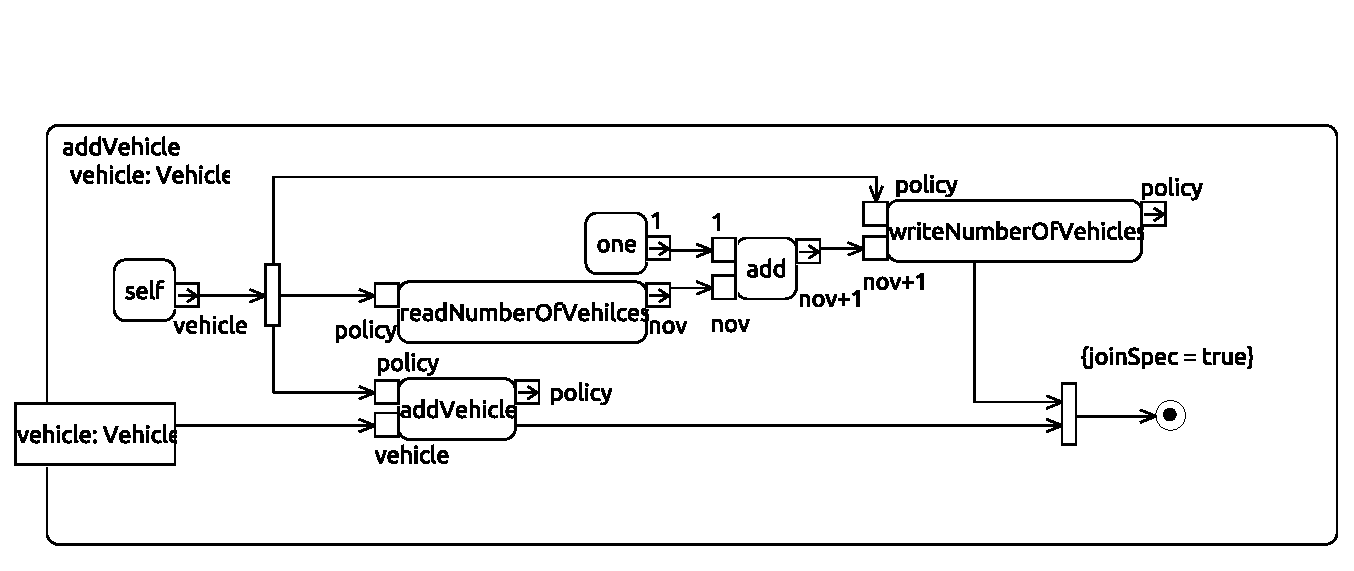
\includegraphics[scale=0.7]{images/insurance_ref/Activity_addVehicle_addVehicle}
 }
 \caption{Activity diagram of operation \texttt{addVehicle} resulting from the refactoring}
 \label{fig:addCarRef}
\end{figure}

\clearpage
\section{Refactoring of fUML models}
\label{sec:fuml-refactoring}
% abstract syntax of fUML and changes in diagrams
% ecore and ocl (with code examples

In the last section we presented an example fUML model comprising a class diagrams and several activity diagrams. We also presented some 
of the possible refactorings such as \textit{extract superclass} on the class diagram and their impact on the activity diagrams. In this 
section we discuss how the syntax of the models actually need to be transformed in order to realize the refactoring. Furthermore we 
describe the refactorings from the prior section in detail.

Every model has two kinds of syntaxes. The concrete syntax (or notation), which defines how the model is visualized, and the abstract
syntax, which defines the UML language elements and the grammar of the model. In order to refactor a model, we need to look 
at its abstract syntax and transform it according to the refactoring rules. Adopting the concrete syntax of co-refactored activity 
diagrams is out of the scope of this work.

Each refactoring takes several parameters that specifies which parts of the model are changed by the refactoring. Additionally each 
refactoring has a precondition and optionally a postcondition. Implementation details are covered in section \ref{sec:toolchain}.

\subsection{Rename class, rename property \& rename operation}
\label{sec:renames}
The rename refactorings need the model element that shall be refactored as well as the new name as parameters. As the abstract syntax 
is not changed the respective classes, operations and properties can then be adapted 
and the changes are automatically propagated. As this is a trivial refactoring we have not explicitly demonstrated it in our example model 
in Figures \ref{fig:classdiagramcomplex} and \ref{fig:classdiagramcomplexRef}. 

In order to guarantee that the 
refactoring is possible, we have to ensure that there are no occurrences of the same type with the same name as the 
new name. In this work we did not take techniques such as operation overloading into account. Listing \ref{lst:renameproperty} shows the 
OCL constraint that has to be checked prior to the \textit{rename property} 
refactoring. Is has to be verified that the names of all inherited properties and the ones of the class itself do not match 
with the indicted new name.

\begin{lstsingle}[language=OCL,caption=OCL for \textit{rename property} refactoring,label=lst:renameproperty]
context Property:
pre:  self.class.attribute.name->
        forAll(n | n <> 'newAttributeName') 
      and 
      self.class.inheritedMember->selectByType(Property).
        name->forAll(n | n <> 'newAttributeName')
\end{lstsingle}

Listing \ref{lst:renameoperation} shows the OCL precondition for the \textit{rename operation} refactoring. As operations 
might have the same name but different parameter declarations we need to test if there exist operations within the 
class or its parents that have the same parameters and the same name as the desired new name of the operation.

\begin{lstsingle}[language=OCL,caption=OCL for \textit{rename operation} refactoring,label=lst:renameoperation]
context Operation:
pre:  self.class.inheritedMember->selectByType(Operation)
        ->forAll(o | (o.parameterableElements() <> 
          self.parameterableElements()) 
          and (o.name <> 'newOperationName')) 
      and 
      self.class.ownedOperation->excluding(self)
        ->forAll(o | (o.parameterableElements() <> 
          self.parameterableElements() 
          and (o.name <> 'newOperationName')))
\end{lstsingle}

As the OCL constraint for the \textit{rename class} refactoring is very similar to one of \textit{rename property} shown 
in Listing \ref{lst:renameproperty} we present it in Appendix \ref{sec:appendix} under Listing \ref{lst:renameclass}.

As we already mentioned the changes are automatically propagated to the respective diagrams. Thanks to this we do 
not need to formulate postconditions for the rename refactorings. The refactoring which we present next will also 
change the model on the abstract syntax level and thus require more thorough pre- and postconditions.

\subsection{Extract superclass}
\label{sec:extract}
The \textit{extract superclass} refactoring is used to extract a superclass out of one or more classes and provide 
a common basis. Most of the time it is used in combination with the \textit{pull up property} and/or the \textit{pull 
up operation} refactoring. In our case the refactoring takes two parameters. The name of the superclass to extract as well as
the class that participates in the refactoring and which will receive the created class as its superclass.

To point out the impacts of a class diagram refactoring on the abstract syntax level we visualize the changes for the 
relevant refactorings. The left hand side of the figures represent the syntax before and the right hand side the syntax 
after the applied refactoring. Concepts that are not affected by the refactoring are colored in gray. 

\begin{figure}
 \makebox[\textwidth]{
  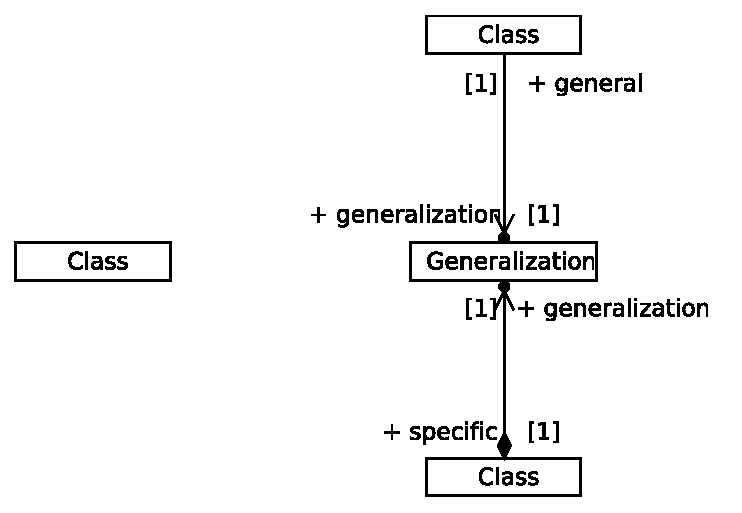
\includegraphics[scale=0.6]{images/extract/Model_Model_Extract}
 }
 \caption{Abstract syntax before \& after \textit{extract superclass} refactoring}
 \label{fig:extract}
\end{figure}

Figure \ref{fig:extract} shows the changes for the \textit{extract superclass} refactoring a new \texttt{Class} is 
introduced and linked via a \texttt{Generalization} to the already existing \texttt{Class}. In our example the two 
classes \texttt{Car} and \texttt{Truck} will be connected to the new superclass \texttt{Vehicle} via the attribute 
\textit{superClass} of the meta-model concept \texttt{Class}. Listing \ref{lst:extractsuperclass}
\footnote{As there are minor differences between the programmatic syntax of OCL in Java and the standard OCL console of Eclipse EMF 
we need to write the term \texttt{uml::} in lowercase letters in Java. You might need to change them to uppercase \texttt{UML::} 
to run the queries within the OCL console in Eclipse EMF.} shows the OCL pre- and 
postcondition for this refactoring. The preconditions checks that there are no classes in the namespace with the 
same name. The postcondition verifies whether the newly created class is visible and the class, from which the refactoring was initiated,
is a subclass. 

Parts of the model\footnote{E.g. the insurance policy could then hold a single variable referencing all vehicles instead 
of one for the cars and one for the trucks.} might also benefit from changing references to the new class, but such a change is not 
trivial and requires additional considerations, which are not covered by this work.

\begin{lstsingle}[language=OCL,caption=OCL for \textit{extract superclass} refactoring,label=lst:extractsuperclass]
context Class:
pre:  self.namespace.member
        ->selectByType(Class).name
        ->forAll(o | o <> 'nameOfClassToExtract')
post: newSuperClass.visibility = uml::VisibilityKind::public
      and 
      self.general->includes(newSuperClass)
\end{lstsingle}

% Fehlende Constraints hinzufuegen
% Zusaetzliche interessante refactorings
% Execution of models (theoretisch, evtl. praktisch)
% Co-refactoring only from class to activity diagrams, not vice versa.
% Refactoring looses concrete syntax representation (e.g. model cannot be opened with papyrus).

\subsection{Pull up property \& pull up operation}
\label{sec:pullup}
Both refactorings are quite similar which is why we describe \textit{pull up property} first and explain the specifics of \textit{pull up 
operation} afterwards. The \textit{pull up property} refactoring gets as parameters the selected property as well as the super class to 
which the property will be moved. Optionally a list of additional properties is provided in the case that more than one property is 
pulled up.

There are two cases of the \textit{pull up property} refactoring. It can either be executed for a property that 
occurs in a single class or in multiple classes where the properties should be combined and pulled up. We consider the single case first. 
The property is a separate object that is only referenced by the class which contains it. To pull it up to the super class it is enough to 
change the containment reference to the super class. No co-refactoring is necessary in this case. However if two or more properties from 
two or more subclasses need to be pulled up to a common super class then this would result in two identical property objects in the super 
class. In this case only one property can be pulled up, and the other properties have to be removed. For each property that is removed a 
co-refactoring of the activities must be performed. The removed property must be replaced by the property that was pulled up to the super 
class in all elements that reference the removed property.

The \textit{pull up operation} refactoring is similar to the \textit{pull up property} variant. The important difference is that
if more than one operation should be pulled up, then not only the operation signatures have to be equivalent, but also the implementation.
However this is hard to verify and outside the scope of this paper, so for pull up operation only one operation can be pulled up at a 
time. Since only one operation is pulled up, it is enough to change the reference to the operation.

The refactorings have several preconditions. There must not already exist a property or an operation with the same name, type or 
multiplicity in the target class and they must not be private. Additionally the specified super class must be a super class of the
class that owns the selected property (or operation). These preconditions are specified in Listing \ref{lst:pullupproperty}. If there are 
additional properties then for each additional property the precondition in Listing \ref{lst:pullupproperty} as well as in Listing 
\ref{lst:additionalproperties} must be satisfied. Listing \ref{lst:additionalproperties} specifies that the additional properties must be
identical to the selected property.

\begin{lstsingle}[language=OCL,caption=OCL for \textit{pull up property},label=lst:pullupproperty]
context Property:
pre: self.class.superClass->select(
         s | s.name = selectedSuperClass.name)->notEmpty()
     and self.visibility <> uml::VisibilityKind::private
     and self.class.inheritedMember->selectByType(Property)
     ->forAll(prop | prop.name = self.name
              and prop.type = self.type
              and prop.upper = self.upper
              and prop.lower = self.lower)
\end{lstsingle}

\begin{lstsingle}[language=OCL, caption={OCL for additional properties}, label=lst:additionalproperties]
context Property:
pre: self.name = otherProperty.name
     and self.type = otherProperty.type
     and self.upper = otherProperty.upper
     and self.lower = otherProperty.lower
\end{lstsingle}

\subsection{Encapsulate property}
\label{sec:encapsulate}
The \textit{encapsulate property} refactoring is more complex than the previous refactorings. The goal is to change the visibility of a 
property to \textit{private} and introduce \textit{public} getter and setter operations to access the value of the property. 

\begin{figure}
 \makebox[\textwidth]{
  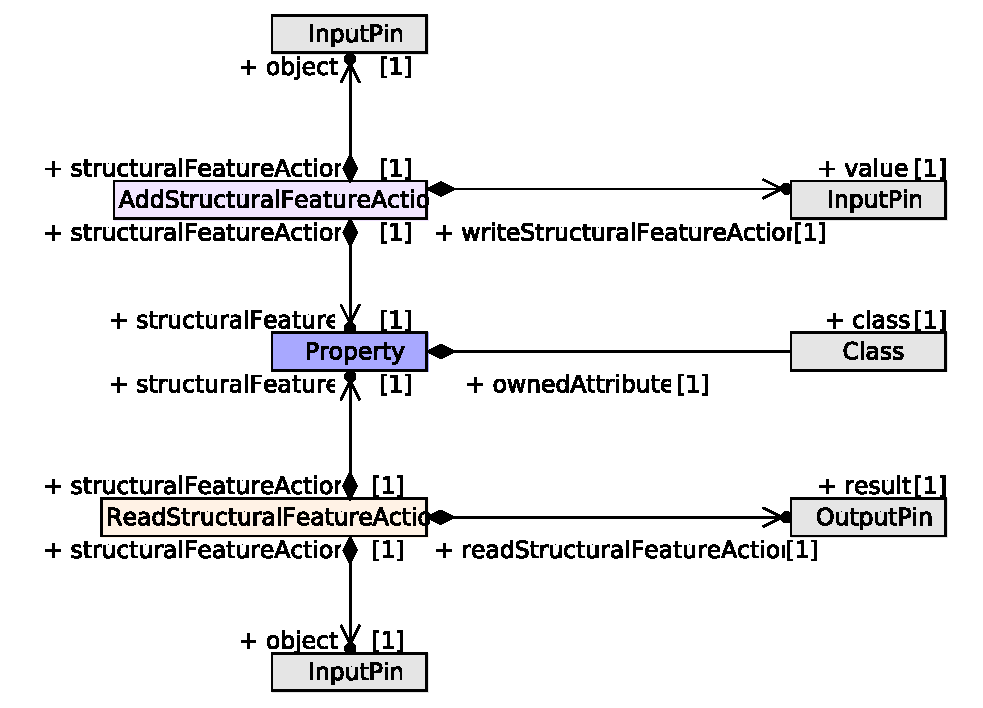
\includegraphics[scale=0.65]{images/encapsulate/Model_Model_Before}
 }
 \caption{Abstract syntax before \textit{encapsulate property} refactoring}
 \label{fig:encapsulatebefore}
\end{figure}

Figure \ref{fig:encapsulatebefore} shows the abstract syntax of a part of the model before the refactoring, 
Figure \ref{fig:encapsulateafter} shows the abstract syntax of the same model after the refactoring\footnote{
In Figure \ref{fig:encapsulateafter} 
we have omitted the activity objects and their internal representation for the sake of visual simplicity. So for each operation 
there is actually a corresponding \texttt{Activity} object, which is also contained by the \texttt{Class}.}.

At first 
getter and setter operations for the property are created and
added to the class. For both operations the corresponding activities are generated and their specification is set to the 
respective operation.
Creating the two activities for the getter and the setter is not trivial as we also need to implement their internal logic. This requires 
the creation of
a \texttt{Read\-Self\-Action} to retrieve the properties owner class and the creation of the correct \texttt{Structural\-Feature\-Action}.
Additionally object and control flow edges, input and output pins and activity parameter nodes need to be created and connected with the 
actions. For each of these elements there are several properties in the abstract syntax that have to be set correctly, such as the 
\textit{type} property of pins or the \textit{source} and \textit{target} properties of edges. If only a single element is not correctly 
generated by the refactoring, then the refactoring results in an incorrect model.

Afterwards each \texttt{Structural\-Feature\-Action} in the model has to be checked, whether it accesses 
the property, and in that case it must be replaced by a \texttt{Call\-Operation\-Action}. If the action is a 
\texttt{Read\-Structural\-Feature\-Action} then the call operation invokes the getter, if the node is of class 
\texttt{Add\-Structural\-Feature\-Value\-Action} the setter operation has to be used. 
One important step is to reassign the corresponding \texttt{InputPin}s and \texttt{OutputPin}s of the original 
actions to the new actions as well as additional activity edges such as \texttt{ObjectFlow}s or \texttt{ControlFlow}s.
Finally the property's visibility is set to private.

\begin{figure}
 \makebox[\textwidth]{
  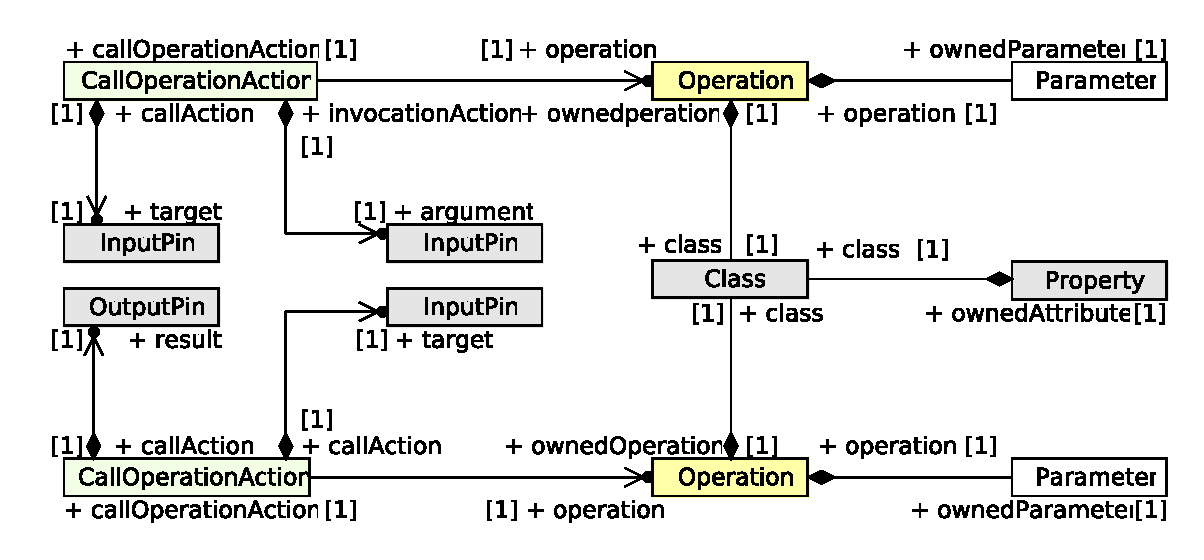
\includegraphics[scale=0.63]{images/encapsulate/Model_Model_After}
 }
 \caption{Abstract syntax after \textit{encapsulate property} refactoring}
 \label{fig:encapsulateafter}
\end{figure}

% TODO: Our example does not contain an operation which uses the encapsulated property of Vehicle.

There are several constraints that need to be checked in order to verify that the refactoring preserved the behavior of the model. 
We present the relevant constraints in Appendix \ref{sec:appendix} in Listing \ref{lst:encapsulate}.
The precondition for this refactoring is that the property is not already private and there are not already getters 
and setters for it. It this case the conditions are not purely formulated in OCL as the \texttt{is\-Distinguishable\-From} method 
demands an element that already exists. We provide this by creating the element before the precondition check and using it 
within our Java refactoring implementation. In case the precondition check fails we simply drop the element. An example how 
to do this is given in Section \ref{sec:toolchain}. 
As UML does not explicitly distinguish between scalars and list types and the differences is only visible
in the multiplicity of the property, the refactoring needs to take this into account. Our current implementation only handles
scalars properties. So additionally the multiplicity of the property must be '1' to prevent the refactoring for list types. We also reject 
the refactoring if \texttt{Clear\-Structural\-Feature\-Action}s or \texttt{Remove\-Structural\-Feature\-Value\-Action}s are present for 
the property as these would also require additional consideration in the refactoring code.

As the postcondition is more complex we have split it into five separate conditions. We verify that the amount of input and output 
pins from the removed structural feature actions matches the number of respective pins of the added call operation actions. Additionally
we require that the type of each pin is correctly set.

%TODO: explain and state ocl constraints for: 
%   * Extract class
%   * Pull up association end
%   * Remove unused class

\clearpage
\section{Toolchain and implementation}
\label{sec:toolchain}
In the last section we explained some refactorings in detail with their respective preconditions and postconditions the model. 
We also discussed which steps have to be taken to actually co-refactor an activity diagram if changes are implied by refactoring 
the class diagram. In this section we will present implementation details as well as a toolchain that allows the integration and 
execution of the refactorings in Eclipse\footnote{\url{http://www.eclipse.org/}}.

\begin{figure}
 \makebox[\textwidth]{
  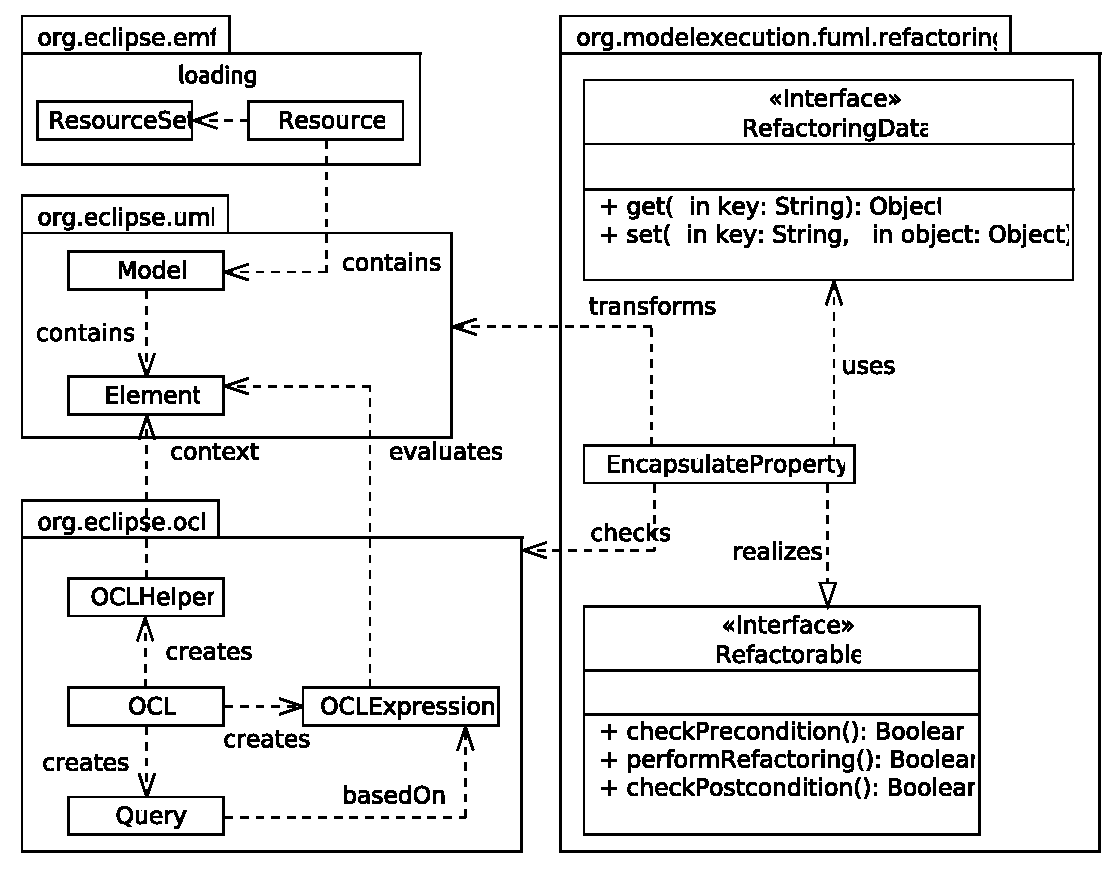
\includegraphics[scale=0.6]{images/Model_Model_Toolchain}
 }
 \caption{Implementation dependencies and class structure}
 \label{fig:toolchain}
\end{figure}

The examples in this work were created in Eclipse with the \textit{Eclipse Modeling Framework} \cite{Steinberg:2009:EEM:1197540} 
(EMF) and Papyrus, a visual modeling tool for different types of diagrams and modeling languages, which stores the models 
in \textit{XML Metadata Interchange} \cite{man:XMI} (XMI) format. We use Java as programming language to manipulate 
the models according to the defined refactorings. The relevant dependencies used for the implementation of the refactorings 
as well as our class structure is depicted in Figure \ref{fig:toolchain}.

% For our toolchain we have relied on the moliz\footnote{http://www.modelexecution.org} repository, mainly for the ability to execute the fUML 
% models in a virtual machine.
\subsection{Model loading}
The \texttt{Resource\-Set} which serves as a basis to read the XMI files needs to be 
initialized first to use the correct settings for UML models. It then can be used to retrieve a \texttt{Resource} object through 
an \texttt{URI}, which is then used to access the different objects in the model. Listing \ref{lst:resourceset} which is contained 
in Appendix \ref{sec:applistings} shows how a model can be initialized and loaded.
All elements contained in the model are instances of Ecore\footnote{The EMF core meta-model implementation of
the MOF meta-meta-model} and they represent classes of the UML meta-model, which is implemented with Ecore.

\begin{lstsingle}[language=Java,caption=Loading elements from the model,label=lst:loadingelements]
Object loadElement(String qualifiedName, 
  java.lang.Class<? extends NamedElement> clazz) {
  
  TreeIterator<EObject> iterator = 
    resource.getAllContents();
  while (iterator.hasNext()) {
    EObject eObject = iterator.next();
    if (!(eObject instanceof NamedElement)) {
      continue;
    }
    if (!clazz.isAssignableFrom(eObject.getClass())) {
      // inspected element is not from target class type
      continue;
    }
    NamedElement element = (NamedElement) eObject;
    if (qualifiedName.equals(element.getQualifiedName())) {
      return eObject;
    }
  }
  return null;
}
\end{lstsingle}

Model elements can be loaded in different ways. We decided to use the qualified name and the class of the concept as 
parameters to identify and load an element. Listing \ref{lst:loadingelements} shows that we first build up a tree of 
the model which is retrieved from the \texttt{Resource}. Then we iterate through the tree and check whether the element 
is a \texttt{NamedElement}. If this is the case we need to verify that element is assignable to the class we want to 
load and that the qualified name is the same. The resulting \texttt{EObject} is returned and needs to be casted by the 
calling method.

\subsection{Model refactoring}
Each of our refactorings is implemented in a separated Java class, which for the demonstration of our implementation 
is initialized and executed by a \textit{JUnit} test\footnote{\url{http://junit.org/}}.
The Java classes representing a refactoring implement the \texttt{Refactorable}
interface that has three operations \texttt{check\-Precondition}, \texttt{perform\-Refactoring}, and \texttt{check\-Post\-condition} as 
shown in Figure \ref{fig:toolchain}. These three methods are executed in the described order to apply the refactoring. 
In the following paragraphs we will explain what is done by the single operations. In order to get a better insight we will 
append Listing \ref{lst:extractSuperclass} which contains the source code for the \textit{extract superclass} refactoring.

First the initialization in the JUnit test identifies and loads the passed model elements that participate in the refactoring with the \texttt{loadElement} 
method introduced in Listing \ref{lst:loadingelements} and puts them into a \texttt{RefactoringData} container 
(Listing \ref{lst:extractSuperclassTest}, line 7-10). It then creates the specific implementation of the \texttt{Refactorable} interface 
and passes the data container as argument (line 12-13). The refactoring implementation creates and evaluates the OCL 
preconditions corresponding to the refactoring on these elements. The class \texttt{OCL} from the \texttt{org.\-eclipse\-.ocl} package is 
used to create and check the constraints as can be seen in Listing \ref{lst:extractSuperclass} lines 38 to 47. Depending on our refactoring the constraint 
can also contain a placeholder (line 13-15) which is later defined as a variable (line 110-115) and then replaced by a specific value 
(line 121-122).

% how to apply queries and changes?
% how to load models?
It is also possible to formulate some of these constraints directly on the model in Java code by checking properties of the abstract syntax
and not use the \textit{OCL} validation facilities. One example is the constraint that verifies that the new super class does not
yet exist in the model (Listing \ref{lst:extractSuperclass}, line 65).

If the preconditions are satisfied the actual refactoring is performed through a direct modification of the model object.
For the \textit{extract superclass} refactoring a new \texttt{Class} instance with the name of the new superclass is created 
and added to the model (Listing \ref{lst:extractSuperclass}, line 61-62). Then the class from which the refactoring classes 
of the model are filtered to select the ones that receive the new generalization, and the newly create superclass is added 
(line 74-77).

After the model is adapted the defined postconditions are checked in the \texttt{checkPostCondition} method 
(Listing \ref{lst:extractSuperclass}, line 97) in the same way as the preconditions. Every of these steps is verified to succeed 
via JUnit as in Listing \ref{lst:extractSuperclassTest} lines 16, 23 and 29.

\subsection{Model execution}
\label{sec:execution}
% usage of fUML reference implementation of BIG
% how to execute models?
In the prior section we discussed how the models are statically examined with \textit{OCL} constraints if a refactoring 
is applicable. In this section we will show how the models can be tested dynamically by executing them. We use the 
reference implementation as described in \cite{DBLP:conf/models/MayerhoferLK12} to execute the activity diagrams of 
our models.

\begin{lstsingle}[language=Java,caption=Converting the UML diagram to fUML,label=lst:conversion]
NamedElement namedElement = obtainFirstNamedElement();
IConverter converter = getConverter(namedElement);
IConversionResult conversionResult = converter
  .convert(namedElement);
Activity activity = conversionResult.getActivity(name);
\end{lstsingle}

Our models are formally created in \textit{UML} and are converted to \textit{fUML} with the \texttt{UML2fUML} converter 
provided by the implementation as shown in Listing \ref{lst:conversion}. The resulting \textit{fUML} diagram is executed in the 
virtual machine for model execution. 
We test our models by examining if a complete execution trace is possible for the chosen activity. Listing \ref{lst:execution} 
shows how the activity is executed step by step. The \texttt{EventListener} catches the event which is created for each 
activity step and builds up a trace. If a trace is created and the process of execution is not interrupted we consider the 
test as successful. Testing more than one trace as some kind of branching is not part of this work and may be included in future studies.

\begin{lstsingle}[language=Java,caption=Executing the activity stepwise and getting the execution trace,label=lst:execution]
getExecutionContext().addEventListener(
  new ExecutionEventListener() {
  @Override
  public void notify(Event event) {
    System.out.println(event);
    if (event instanceof ActivityEntryEvent 
      && executionID == -1) {
      executionID = ((ActivityEntryEvent) event)
          .getActivityExecutionID();
    }
    if (event instanceof SuspendEvent) {
      SuspendEvent suspendEvent = (SuspendEvent) event;
      getExecutionContext().resume(
          suspendEvent.getActivityExecutionID());
    }
  }
});
getExecutionContext().executeStepwise(activity, null, 
  new ParameterValueList());
getExecutionContext().getTrace(executionID);
\end{lstsingle}

In the process of refactoring before and after each model change the corresponding activities are executed to prove that 
the refactoring did not corrupt the model. 
%TODO: we cannot actually prove anything. Because we cannot show that the execution trace goes through all branches that 
%have been affected by the changes. Or can we?
Further testing can be implemented by going through the trace and verifying 
that every node of the trace has the expected values.

\subsection{Eclipse Integration}
\label{sec:guiintegration}
In this section we discuss how we can integrate the defined refactorings to the Eclipse framework. For our further 
research we plan to implement some the refactorings in EMF Refactor. EMF Refactor is an Eclipse incubation project 
which focuses on static model analysis and refactoring.

EMF Refactor analyses a project for so called code smells and calculates common model metrics. Those two project quality 
indicators reflect in a very convenient way which parts of a model could be improved. From a report view different 
refactorings already implemented in EMF Refactor can be applied to change the model. The refactorings work in the UML tree 
editor as well as in several graphical editors based on EMF.

However EMF Refactor mainly supports the refactoring of class diagrams. The effects that can be seen in activity diagrams 
when refactoring class diagrams are error prone and seem to happen more or less by accident. Nevertheless we intend to 
implement our above mentioned catalog in EMF Refactor because of the good integration with the Eclipse framework, the 
easy generation of simple refactorings\footnote{The framework supports the generation of new smells, metrics and 
refactorings with a module wizard in Eclipse.} and the various implementation possibilities\footnote{EMF Refactor 
supports the creation of refactorings in \textit{Java}, \textit{OCL} and \textit{Henshin} a transformation language.}.

\section{Current limitations}
\label{sec:limitations}
Our work currently has several limitations. So far we have designed a set of related class and activity diagrams,
which are the basis for our refactorings. We have discussed the \textit{extract superclass} refactoring including its
pre- and post conditions and shown how it can be refactored with our toolchain. Until the final version of this
paper we will formulate the pre- and postconditions for some of the refactorings that have not yet been discussed.
Furthermore we will implement several more refactorings from the list shown in Figure \ref{fig:refactoringlist}, such as the
\textit{extract class}, the \textit{rename operation}, the \textit{pullup operation}, the \textit{pullup field} and 
\textit{rename variable} refactorings.

When the paper was written the refactorings were not yet implemented in EMF Refactor.
We plan to create the whole refactoring chain for \textit{extractSuperclass} in EMF Refactor which includes extracting 
a super class and pulling up the properties and operations programmatically. We also take the co-refactoring of the activity 
diagrams into account. If this works as intended we plan to rewrite the creation wizard which allows only refactorings 
on a single class. The code should ideally be carried to the EMF Refactor repository after a quality review.

\section{Related work}
\label{sec:relatedwork}
% Refactoring of prgram code

In this section we give an overview on the related work. Refactoring in a general way with preconditions was described
by Opdyke \cite{mast:REFOOF} in his master thesis and stated more precisely by Roberts \cite{rob99} who also introduced
postconditions for refactorings. Fowler \cite{fow99} generated an extensive yet simple to understand catalog of
refactorings for Java and Ruby which can be be adapted to model refactorings.

% Refactoring of models and OCL Code analysis via OCL

Suny{\'e} et. al. \cite{DBLP:conf/uml/SunyePTJ01} described how several refactorings can be applied to \textit{UML}
diagrams and introduced OCL as a possiblity to specify pre- and postconditions. Gorp \textit{et al.} \cite{gorp03} extends the
discussion with the usage of \textit{OCL} for additional analysis such as code smells of models.

% Code execution via fUML

Despite of the further discussion of model refactoring (\cite{DBLP:conf/uml/CorreaW04}, \cite{DBLP:conf/ershov/BaarM06},
\cite{DBLP:journals/ase/ArendtT13}) most authors concentrate on static analysis and class diagram representations of
models. Dynamic analysis of models by execution and debugging \textit{fUML} models is discussed by Mayerhofer
\cite{DBLP:conf/icse/Mayerhofer12} and provides the basis for the approach discussed here. Mayerhofer \textit{et al.}
\cite{DBLP:conf/models/MayerhoferLK12} furthermore introduce a runtime model and an
implementation\footnote{http://www.modelexecution.org} that is capable to test the models and directly show impacts of
refactorings.

% Refactoring implementation with EMF Refactor

Arendt and Taentzer \cite{DBLP:journals/ase/ArendtT13} present a framework that is based on \textit{Eclipse} and the
\textit{Eclipse Modelling Framework} which allows static model analysis and refactorings that are implemented in
different languages (Java, OCL \& Henshin) and can be directly extended in \textit{Eclipse}.


\section{Conclusion}
\label{sec:conclusion}
Refactoring models is a rather difficult task and it requires a concise knowledge of the involved technologies, with
the list of involved technologies being rather long. For one a reasonably well understanding of fUML is required, in
particular how class diagrams and activity diagrams are constructed and how they are related. It is not enough to simply
be able to draw both class and activity diagrams, as one also needs a good understanding of the meta-meta-model (MOF) and
the fUML and UML meta-model implementations in Ecore in order to understand and manipulate the model on the level of its 
abstract syntax. Finally an understanding of EMF (in particular Ecore and OCL) is required. While MOF and OCL are both 
modeling concepts and languages respectively, EMF contains implementations for them in Java with a complex API. 
Understanding these APIs of Ecore and OCL is required to perform the refactorings and was a prerequisite to build
our toolchain.

While it took a considerable amount of time to get familiar with all these technologies, we were eventually able to
create a tool chain for model refactoring. With the toolchain in place another challenge was to identify the required 
steps to perform the actual refactoring work. In particular this meant to identify how the activity diagrams need to 
change if a change is made in the class diagram.

Most of our efforts in the development of this work were focused on gaining a comprehensive understanding of the
technologies described above, to develop the tool chain and to draw the various diagrams presented in this paper and make 
them executable. We have presented a comprehensive set of diagrams as the basis for our refactoring work and demonstrated 
the feasibility of our tool chain. However a more comprehensive evaluation of the different refactorings including the 
specification of pre- and postconditions OCL in is still required and will be the focus of our ongoing efforts.

\newpage
\bibliographystyle{acm}
\bibliography{references}

\newpage
\appendix
\section{Appendix}
\label{sec:appendix}

\subsection{OCL Constraints}
\label{sec:appconstraints}

\begin{lstsingle}[language=OCL,caption=OCL for \textit{rename class} refactoring,label=lst:renameclass]
context Class:
pre:  self.namespace.member
      ->selectByType(Class)
      ->forAll(c | c.name <> 'newClassName')
\end{lstsingle}
\\
\begin{lstlisting}[language=OCL,caption=OCL for \textit{encapsulate property} refactoring,label=lst:encapsulate]
context Property:
pre:  self.visibility <> uml::VisibilityKind::private 
      and 
      self.class.ownedOperation
        ->forAll(o | o.isDistinguishableFrom(setOperation, 
            self.namespace)
          and 
          o.isDistinguishableFrom(getOperation, 
            self.namespace)) 
      and 
      uml::ClearStructuralFeatureAction.allInstances().
        structuralFeature->forAll(s|s<>self)
      and
      uml::RemoveStructuralFeatureValueAction.allInstances().
        structuralFeature->forAll(s|s<>self)
      and
      self.upper <= 1"
post: uml::CallOperationAction.allInstances()
        ->select(action | action.operation = operation)
        ->collect(input)->select(pin | pin <> null)
        ->size() = inputPinCounter
      and
      uml::CallOperationAction.allInstances()
        ->select(action | action.operation = operation)
        ->collect(result)->select(pin | pin <> null)
        ->size() = outputPinCounter
      and
      uml::CallOperationAction.allInstances()
        ->select(action | action.operation = operation)
        ->collect(target)->forAll(target | target.type 
        = self.class)
      and 
      uml::CallOperationAction.allInstances()
        ->select(action | action.operation = operation)
        ->collect(argument)->forAll(argument | argument.type 
        = self.type)
      and
      uml::CallOperationAction.allInstances()
        ->select(action | action.operation = operation)
        ->collect(result)->forAll(result | result.type 
        = self.type)
\end{lstlisting}

\subsection{Code Listings}
\label{sec:applistings}

\begin{lstsingle}[language=Java,caption=Initializing the resourceset,label=lst:resourceset]
void initializeResourceSet() {
  ResourceSet resourceSet = new ResourceSetImpl();
  resourceSet.getPackageRegistry()
    .put(UMLPackage.eNS_URI, UMLPackage.eINSTANCE);
  resourceSet.getResourceFactoryRegistry()
    .getExtensionToFactoryMap().put(
      UMLResource.FILE_EXTENSION, 
      UMLResource.Factory.INSTANCE);
  File file = new File(MODEL_PATH);
  URI uri = URI.createFileURI(file.getAbsolutePath());
  Resource resource = resourceSet
    .getResource(uri, true);
}
\end{lstsingle}
\\

\begin{lstlisting}[language=Java,caption=Execution of the \textit{extract superClass} refactoring as test,label=lst:extractSuperclassTest]
@Test
public void superclassExtration {
  String superClassName = "Vehicle";

  RefactoringData data = new RefactoringDataImpl();
  data.set("newSuperClassName", superClassName);
  Class clazz = 
    (Class) loadElement("Model::insurance::Car", 
    Class.class);
  data.set("selectedElement", clazz);

  Refactorable extractSuperClassRefactoring = 
    new ExtractSuperClassRefactorableImpl(data);

  try {
    assertTrue("Precondition not met!", 
      extractSuperClassRefactoring.checkPreCondition());
  } catch (ParserException pre) {
    fail("Preconstraints failed with ParserException");
  }

  try {
    extractSuperClassRefactoring.performRefactoring();
  } catch (RefactoringException e) {
    e.printStackTrace();
  }

  try {
    assertTrue("Post condition not met!", 
      extractSuperClassRefactoring.checkPostCondition());
  } catch (ParserException post) {
    post.printStackTrace();
    fail("Postconstraints failed with ParserException");
  }

  try {
    resource.save(new FileOutputStream(
      new File(MODEL_SUPERCLASS_PATH)), null);
  } catch (Exception e) {
    e.printStackTrace();
  }
}
\end{lstlisting}

\begin{lstlisting}[language=Java,caption=Source code of the \textit{extract superClass} refactoring,label=lst:extractSuperclass]
public class ExtractSuperClassRefactorableImpl 
  implements Refactorable {

  private final OCL<?, EClassifier, ?, ?, ?, 
    EParameter, ?, ?, ?, Constraint, EClass, EObject> ocl;
  private final OCLHelper<EClassifier, ?, ?, 
    Constraint> helper;

  private static final String OCL_PRE_CONSTRAINT =
    "self.namespace.member->selectByType(Class).name"
    + "->forAll(o | o <> '%s')";

  private static final String OCL_POST_CONSTRAINT = 
    "newSuperClass.visibility = uml::VisibilityKind::public"
    + " and self.general->includes(newSuperClass)";

  private final RefactoringData data;

  public ExtractSuperClassRefactorableImpl(RefactoringData 
    data) {
    this.ocl = 
      OCL.newInstance(EcoreEnvironmentFactory.INSTANCE);
    this.helper = ocl.createOCLHelper();
    this.data = data;
  }

  @Override
  public boolean checkPreCondition() throws 
    ParserException {
    
    helper.setContext(UMLPackage.eINSTANCE.getClass_());

    Class selectedElement = 
      (Class) data.get("selectedElement");
    String newSuperClassName = 
      (String) data.get("newSuperClassName");

    OCLExpression<EClassifier> expression;
    expression = helper.createQuery(String.
      format(OCL_PRE_CONSTRAINT, newSuperClassName));

    Query<EClassifier, EClass, EObject> query = 
      ocl.createQuery(expression);

    if (!query.check(selectedElement)) {
      return false;
    }

    return true;
  }

  @Override
  public boolean performRefactoring() throws 
    RefactoringException {
    
    Class selectedElement = 
      (Class) data.get("selectedElement");
    String newSuperClassName = 
      (String) data.get("newSuperClassName");
    Package pkg = selectedElement.getPackage();

    Class superClass = UMLFactory.eINSTANCE.createClass();
    superClass.setName(newSuperClassName);

    if (pkg.getPackagedElement(newSuperClassName) == null) {
      // the owning package does not own a class with the 
      // inserted name create new class named 'className'
      Class newSuperclass = 
        UMLFactory.eINSTANCE.createClass();
      newSuperclass.setName(newSuperClassName);
      pkg.getPackagedElements().add(newSuperclass);
      // create generalization from context class to 
      // new class
      Generalization gen = 
        UMLFactory.eINSTANCE.createGeneralization();
      selectedElement.getGeneralizations().add(gen);
      gen.setGeneral(newSuperclass);
      data.set("newSuperClass", newSuperclass);
    } else { 
      // the owning package owns a class with the 
      // inserted name
      Class existingClass = 
        (Class) pkg.getPackagedElement(newSuperClassName);
      // create generalization from context class 
      // to existing class
      Generalization gen = 
        UMLFactory.eINSTANCE.createGeneralization();
      selectedElement.getGeneralizations().add(gen);
      gen.setGeneral(existingClass);
      data.set("newSuperClass", existingClass);
    }

    return true;
  }

  @Override
  public boolean checkPostCondition() throws 
    ParserException {
    
    helper.setContext(UMLPackage.eINSTANCE.getClass_());

    Class selectedElement = 
      (Class) data.get("selectedElement");
    Class superClass = (Class) data.get("newSuperClass");

    if (superClass == null) {
      return false;
    }

    Variable<EClassifier, EParameter> variable = 
      ExpressionsFactory.eINSTANCE.createVariable();
    variable.setName("newSuperClass");
    variable.setType(UMLPackage.Literals.CLASSIFIER);
    ocl.getEnvironment().addElement(variable.getName(), 
      variable, true);

    OCLExpression<EClassifier> expression = 
      helper.createQuery(OCL_POST_CONSTRAINT);
    Query<EClassifier, EClass, EObject> query = 
      ocl.createQuery(expression);
    query.getEvaluationEnvironment().add("newSuperClass", 
      superClass);
    if (!query.check(selectedElement)) {
      return false;
    }

    return true;
  }
}
\end{lstlisting}

\end{document}
